\subsection{Content Server} \label{section:counter-replace-server}
This appraoch enforces users to login on a server, but not to get their verification response but to get part or all of the content of the application.
Content cannot be guessed by \gls{luckypatcherg}.
\newline
\begin{figure}[h]
    \centering
    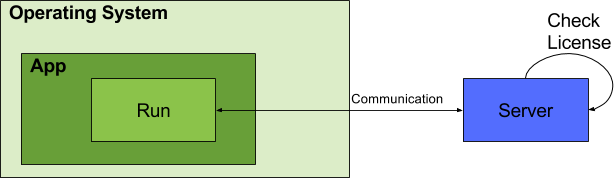
\includegraphics[width=0.8\textwidth]{data/contentServer.png}
    \caption{Abstraction of an application and a content server}
    \label{fig:contentServer}
\end{figure}
An implementation can be illustrated by looking at the application Spotify \cite{spotify} as an example.
Instead of verifying the license locally on the device, the user has to enter his credentials and send them to the server.
In case the credentials are valid, the user has the right to receive content.
The content, the music in this case, is no longer on the phone itself, but streamed from the server.
The attacker still can circumvent the login process inside the application by manipulating the code.
Since the content is on the server and the user has to be authorized on it, no content is available inside the application.
Thus attacks on the applications itself do not work anymore.
\newline
\newline
In general, a content server is a solution against piracy, but it has downsides as well.
The first problem is that this architecture cannot be applied to all applications.
If there is no complex enough content that can be moved to the server, it doesn't work.
\newline
The second problem is the more complex overall architecture.
Instead of using Google’s solution for handling the verification, a client server structure for the content has to be developed and implemented.
\newline
The third problem are the additional resources needed.
When outsourcing parts of the application on a server, money is needed for the server.
\newline
The fourth problem is the requirement for a permanent online connection.
It limits the freedom of users and creates additional internet traffic and costs.
This is not accepted by all users.
\newline
\newline
This mechanism protects the developers \gls{ip} when the core algorithm is moved to the server.
This prevents attackers not only from using the application for free, but also from reconstructing the the core functionality and implementing it somewhere else.
